\usetikzlibrary{arrows.meta}



\definecolor{lineBlue}{RGB}{57,106,177}
\definecolor{lineOrange}{RGB}{218,124,48}
\definecolor{lineGreen}{RGB}{62,150,81}
\definecolor{lineRed}{RGB}{204,37,41}
\definecolor{lineGray}{RGB}{83,81,84}
\definecolor{linePurple}{RGB}{107,76,154}
\definecolor{lineMaroon}{RGB}{146,36,40}
\definecolor{barBlue}{RGB}{114,147,203}
\definecolor{barOrange}{RGB}{225,151,76}
\definecolor{barGreen}{RGB}{132,186,91}
\definecolor{barRed}{RGB}{211,94,96}
\definecolor{barGray}{RGB}{128,133,133}
\definecolor{barPurple}{RGB}{144,103,167}
\definecolor{barMaroon}{RGB}{171,104,81}


\begin{figure}
    \centering

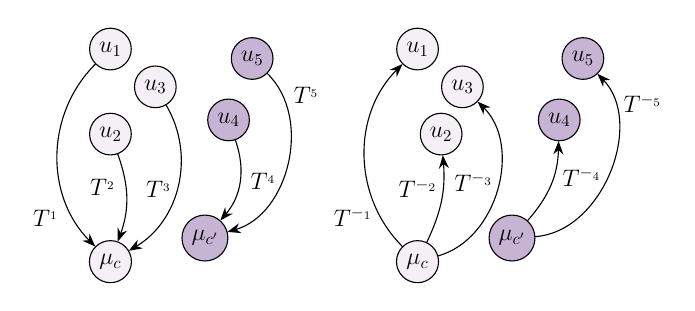
\begin{tikzpicture}[scale=0.6, every node/.style={transform shape}]

% Left figure (forward alignment)
\begin{scope}[every node/.style={circle,draw,minimum size=10,transform shape, font=\Large}]
    \node[fill=barPurple!10] (q2) at (-0.5,5.7) {$u_2$};
    \node[fill=barPurple!10] (q1) at (-0.5,7.5) {$u_1$};
    \node[fill=barPurple!10] (q3) at (0.45,6.7) {$u_3$};
    \node[fill=barPurple!50] (q4) at (2,6) {$u_4$};
    \node[fill=barPurple!50] (q5) at (2.5,7.3) {$u_5$};

    
    \node[fill=barPurple!10] (A) at (-0.5,3) {$\mu_c$};
    \node[fill=barPurple!50] (B) at (1.5,3.5) {$\mu_{{c'}}$};
\end{scope}


\begin{scope}[>={Stealth[black]},
              every edge/.style={draw=black, transform shape, font=\Large}]
    \path [->] (q1) edge[bend right=45] 
    node[label={$ T^{\btheta_1}$}, shift={(-0.25,-1.75)}] {} (A);
        \path [->] (q2) edge[bend left=20] 
    node[label={$ T^{\btheta_2}$}, shift={(-0.5,-0.2)}] {} (A);
        \path [->] (q3) edge[bend left=45] 
    node[label={$ T^{\btheta_3}$}, shift={(-0.4,-0.5)}] {} (A);
    \path [->] (q4) edge[bend left=30] 
    node[label={$ T^{\btheta_4}$}, shift={(0.5,-0.4)}] {} (B);
    \path [->] (q5) edge[bend left=60] 
    node[label={$ T^{\btheta_5}$}, shift={(0.4,1)}] {} (B);
\end{scope}


% Right figure (backward alignment)
\def\offset{6.5}
\begin{scope}[every node/.style={circle,draw,minimum size=10,transform shape, font=\Large}]
    \node[fill=barPurple!10] (U2) at (0+\offset,5.7) {$u_2$};
    \node[fill=barPurple!10] (U1) at (-0.5+\offset,7.5) {$u_1$};
    \node[fill=barPurple!10] (U3) at (0.45+\offset,6.7) {$u_3$};
    \node[fill=barPurple!50] (U4) at (2.5+\offset,6) {$u_4$};
    \node[fill=barPurple!50] (U5) at (3+\offset,7.3) {$u_5$};

    
    \node[fill=barPurple!10] (A) at (-0.5+\offset,3) {$\mu_c$};
    \node[fill=barPurple!50] (B) at (1.5+\offset,3.5) {$\mu_{{c'}}$};
\end{scope}

\begin{scope}[>={Stealth[black]},
              every edge/.style={draw=black, transform shape, font=\Large}]
    \path [<-] (U1) edge[bend right=45] 
    node[label={$ T^{-\btheta_1}$}, shift={(-0.25,-1.75)}] {} (A);
        \path [<-] (U2) edge[bend left=15] 
    node[label={$ T^{-\btheta_2}$}, shift={(-0.5,-0.2)}] {} (A);
        \path [<-] (U3) edge[bend left=60] 
    node[label={$ T^{-\btheta_3}$}, shift={(-0.5,-0.3)}] {} (A);
    \path [<-] (U4) edge[bend left=20] 
    node[label={$ T^{-\btheta_4}$}, shift={(0.65,-0.3)}] {} (B);
    \path [<-] (U5) edge[bend left=65] 
    node[label={$ T^{-\btheta_5}$}, shift={(0.7,1)}] {} (B);
\end{scope}
\end{tikzpicture}
    \subcaptionbox{Centroids computed using forward warps\label{Fig:Intro:Left}}[0.45\linewidth]{}
    \hfill
    \subcaptionbox{The ICAE loss computed using backward warps\label{Fig:Intro:Right}}[0.45\linewidth]{}
\caption{The Inverse Consistency Averaging Error loss in a two-class example. 
(a) The signals $u_1$, $u_2$, and $u_3$ are in class $c$; $u_4$ and $u_5$ are in class $c'$. Within each class, the centroid
($\mu_c$ or $\mu_{{c'}}$) is obtained by averaging the warped signals ($(u_i\circ T^{\btheta_i})_{i\in\set{1,2,3}}$
or $(u_i\circ T^{\btheta_i})_{i\in\set{4,5}}$)
using the forward warps. (b) The loss is computed using the backward warps; \ie, 
we measure dissimilarity between each $u_i$ and its class centroid, where the latter is first warped backward (``unwarped") using $T^{-\btheta_i}$ (the inverse of $T^{\btheta_i}$). 
}
\label{fig:icae:example}
\end{figure}
